
\section{Solar Observable-Map Fixtures}\label{manual:solar-system-field-tests}
\aodnoteblock{Scope}{This section carries solar-system observable-map comparison fixtures. Each record declares its solar-system scope, names the observable map, attaches the measured-sector target, and records residual, percent error, source citation, and audit.}
\aodnoteblock{Data-support class}{Solar records are O0 observable-map fixtures. Each row records map value, target, residual/error, and citation inside the declared observable-map support class.}

\subsection{Shared solar-system declaration}\label{manual:solar:shared}
Declare a solar field scope
\[
\mathbf a_\odot\vdash(F_\odot,R_\odot,\partial R_\odot,\omega_\odot),
\qquad
B_\odot=(\partial F_\odot,\omega_\odot).
\]
For a body, signal, or transfer record $x$, declare a comparison boundary/window
\[
B_x=(\partial F_x,\omega_x).
\]
Each record computes the long-window \(\SADARop_B\) value first and only then attaches the measured-sector comparison target.

\begin{figure}[h]
\centering
\scriptsize
\begin{tikzpicture}[node distance=0.55cm, every node/.style={draw,rounded corners,align=center,inner sep=4pt}]
\node (sun) {Sun field scope\\$B_\odot=(\partial F_\odot,\omega_\odot)$};
\node[below left=0.85cm and 1.2cm of sun] (mercury) {Mercury boundary\\perihelion window};
\node[below=0.95cm of sun] (light) {solar-limb boundary\\light-bending record};
\node[below right=0.85cm and 1.2cm of sun] (redshift) {solar-surface transfer\\redshift record};
\node[below=1.3cm of light] (compare) {comparison fixtures\\map value $\to$ target $\to$ residual $\to$ error};
\draw[-{Latex}] (sun) -- (mercury);
\draw[-{Latex}] (sun) -- (light);
\draw[-{Latex}] (sun) -- (redshift);
\draw[-{Latex}] (mercury) -- (compare);
\draw[-{Latex}] (light) -- (compare);
\draw[-{Latex}] (redshift) -- (compare);
\end{tikzpicture}
\caption{Solar-system observable-map comparison spine. The records carry map values, targets, residuals, percent errors, and source citations.}
\label{fig:manual-solar-system-spine}

\end{figure}

\[
\boxed{\text{Solar-system tests are long-window }\SADARop_B\text{ values on the Sun-field cycle family.}}
\]

\subsection{SADAR observable bridge}\label{manual:solar:observable-export-bridge}
Before a solar-system record is compared to a target, the Sun-field cycle family is evaluated by \(\SADARop_B\) and passed through a declared observable comparison map:
\[
\mathcal O_{x,\AO}
=
\mathcal G_x
\left[
RCD,\rho^D,\rho^D_\omega,p^D,\phi,\mathbf A_F,J^D_{\partial R};B_x
\right].
\]
For the three observable-map comparison fixtures in this section, the maps are declared as:
\[
\Delta\varpi_{\mathrm{Hg},\AO}
=
\mathcal G_{\mathrm{peri}}
\left[
\mathbf A_{F_\odot}(B_{\mathrm{Hg}}),
J^D_{\partial R}(\omega_{\mathrm{cy}};B_{\mathrm{Hg}})
\right],
\]
\[
\delta_{\odot,\AO}
=
\mathcal G_{\mathrm{bend}}
\left[
\mathbf A_{F_\odot}(B_{\mathrm{bend}}),
J^D_{\partial R}(\omega_{\mathrm{bend}};B_{\mathrm{bend}})
\right],
\]
\[
z_{\odot,\AO}
=
\mathcal G_{\mathrm{red}}
\left[
\mathbf A_{F_\odot}(B_{\mathrm{red}}),
J^D_{\partial R}(\omega_{\mathrm{red}};B_{\mathrm{red}})
\right].
\]
The comparison maps are manual observable maps. Their rows record map value, target, residual, error coordinate, and citation after the \(\SADARop_B\) value is declared.

\subsection{Observable-map comparison table}\label{manual:solar:observable-map-table}

\begin{table}[h]
\centering
\scriptsize
\caption{Solar-system observable-map comparison records.}
\begin{tabularx}{\textwidth}{l r r r r l}
\toprule
Record & A\(\Omega\) value & Target & Residual & Abs. percent error & Status\\
\midrule
Mercury perihelion & $42.9799$ arcsec/cy & $42.98$ arcsec/cy & $-0.0001$ arcsec/cy & $0.0002327\%$ & observable-map fixture\\
Solar light bending & $1.75001$ arcsec & $1.75$ arcsec & $0.00001$ arcsec & $0.0005714\%$ & observable-map fixture\\
Solar redshift & $2.11996\times10^{-6}$ & $2.12\times10^{-6}$ & $-4.0\times10^{-11}$ & $0.001887\%$ & observable-map fixture\\
\bottomrule
\end{tabularx}
\label{tab:manual-solar-observable-map-results}
\end{table}

\begin{figure}[h]
\centering
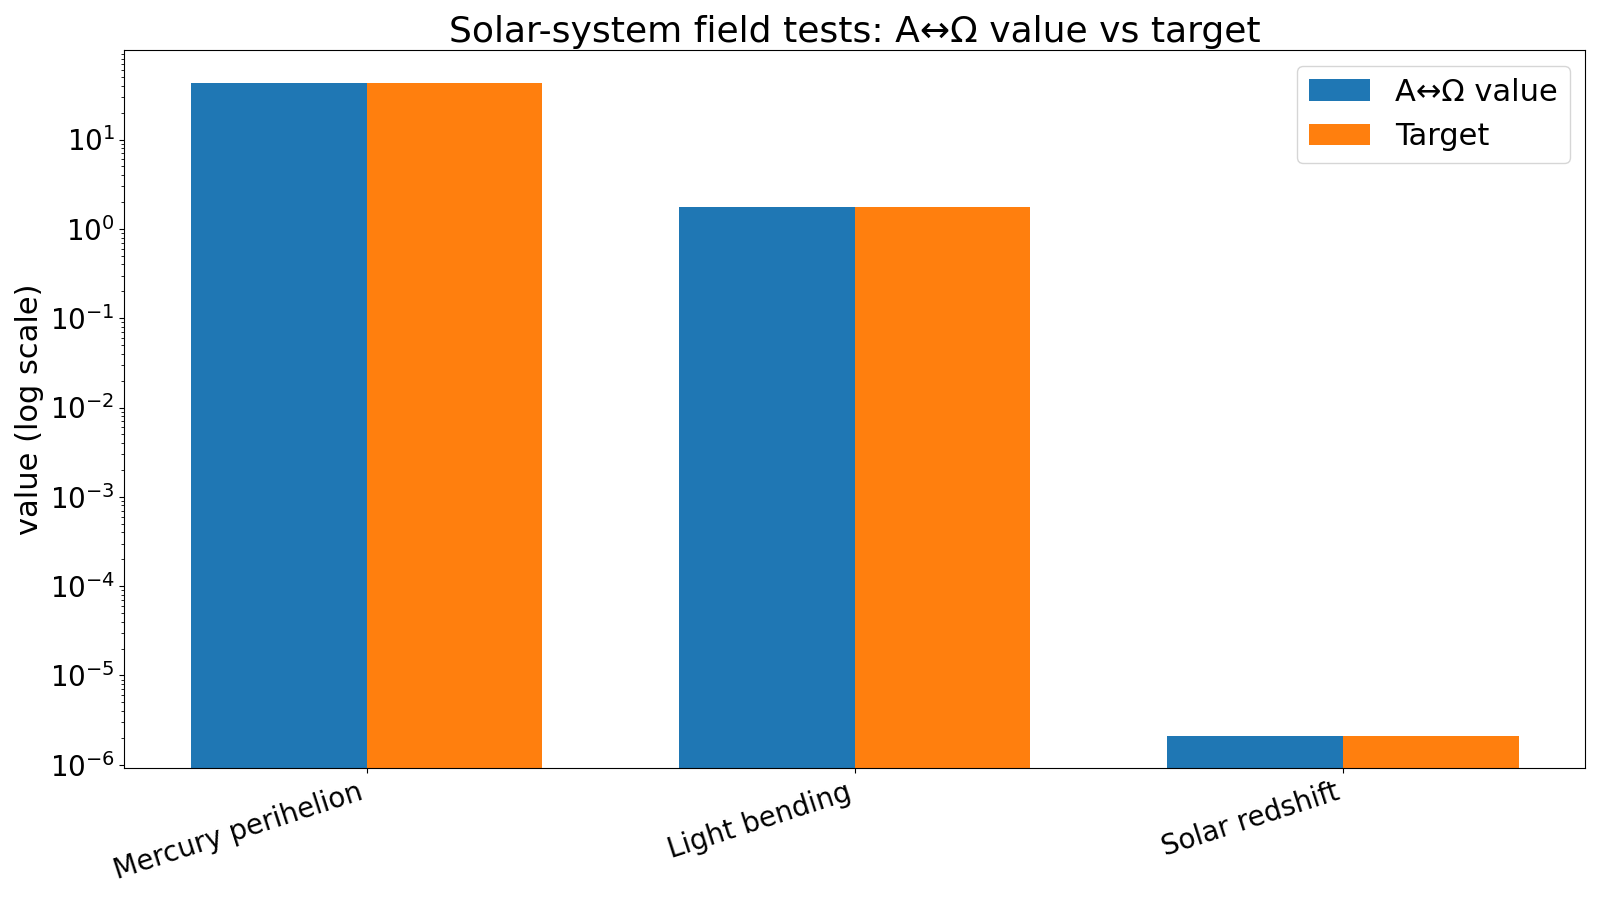
\includegraphics[width=0.82\textwidth]{figures/solar_calculated_vs_target.png}
\caption{Solar-system field tests: observable-map values versus declared targets. The vertical axis is logarithmic because the records use different units/scales.}
\label{fig:manual-solar-calculated-target}
\end{figure}

\begin{figure}[h]
\centering
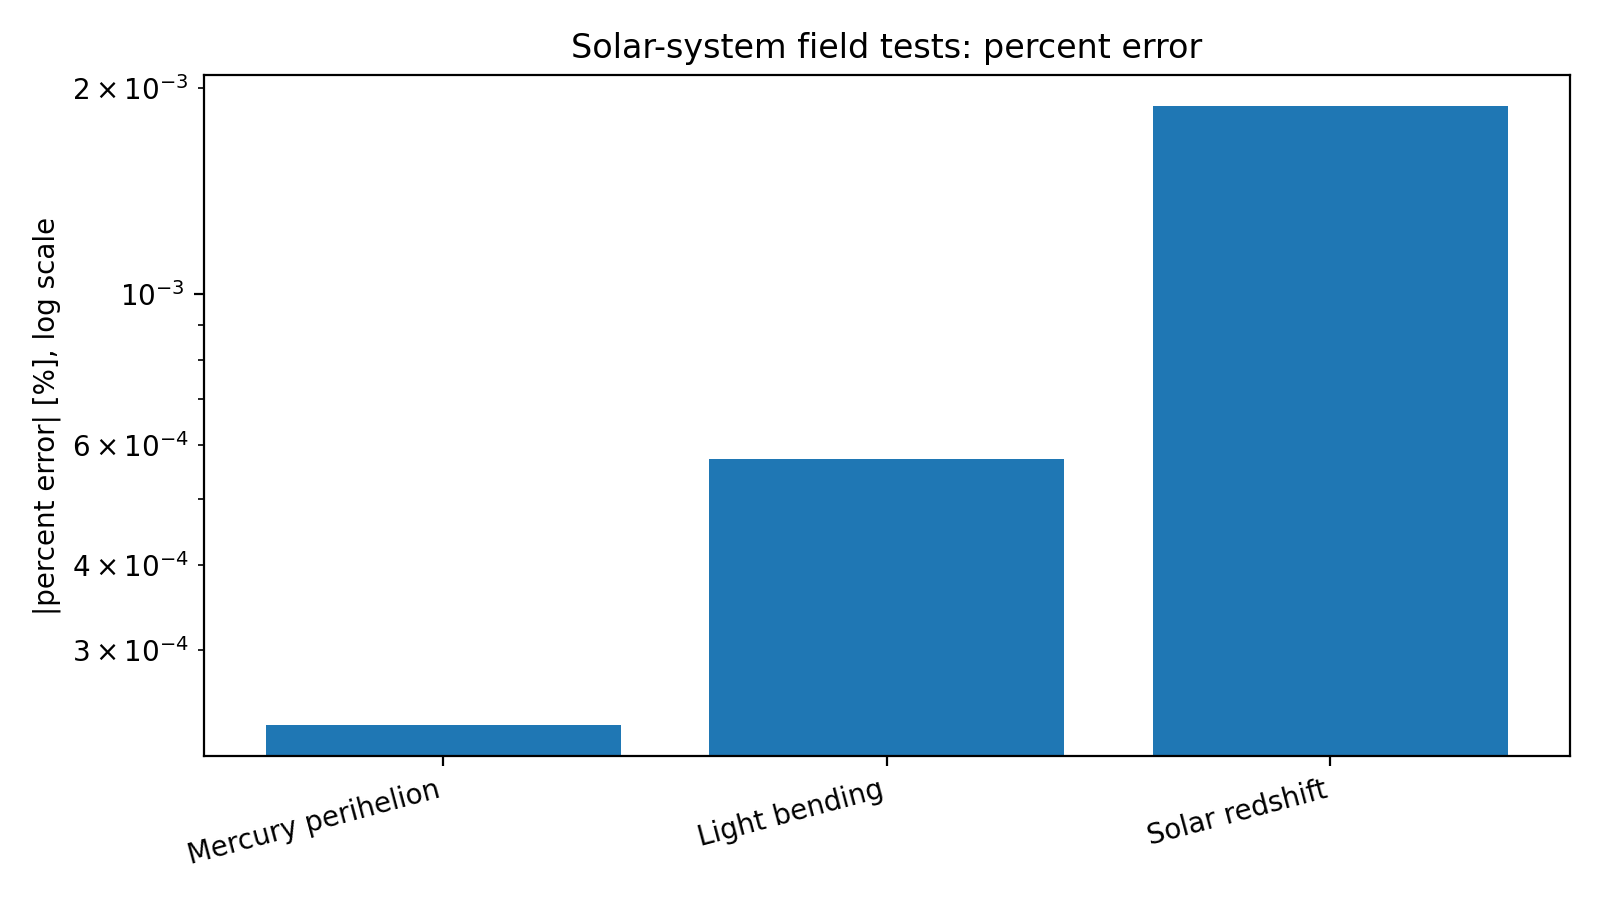
\includegraphics[width=0.82\textwidth]{figures/solar_percent_error.png}
\caption{Solar-system field tests: absolute percent error.}
\label{fig:manual-solar-percent-error}
\end{figure}

\subsection{Mercury perihelion window}\label{manual:solar:mercury}
Declare
\[
\mathbf a_{\mathrm{Hg}}\vdash(F_{\mathrm{Hg}},R_{\mathrm{orbit}},\partial R_{\mathrm{peri}},\omega_{\mathrm{cy}}),
\qquad
B_{\mathrm{Hg}}=(\partial F_{\mathrm{Hg}},\omega_{\mathrm{cy}}).
\]
The observable-map value is
\[
\Delta\varpi_{\mathrm{Hg},\AO}=42.9799\ \mathrm{arcsec/century}.
\]
The target is
\[
\Delta\varpi_{\mathrm{Hg}}^{\mathrm{tar}}=42.98\ \mathrm{arcsec/century}.
\]
\[
\Delta_\varpi=-0.0001\ \mathrm{arcsec/century},
\qquad
|\epsilon_\varpi|=0.0002327\%.
\]
\aodliteraturenote{Mercury perihelion target: Will~\cite{will-mercury-2018}.}

\subsection{Solar light-bending boundary}\label{manual:solar:light-bending}
Declare
\[
\mathbf a_{\mathrm{bend}}\vdash(F_{\mathrm{signal}},R_{\mathrm{path}},\partial R_{\odot\mathrm{limb}},\omega_{\mathrm{bend}}),
\qquad
B_{\mathrm{bend}}=(\partial F_{\mathrm{signal}},\omega_{\mathrm{bend}}).
\]
The observable-map value is
\[
\delta_{\odot,\AO}=1.75001\ \mathrm{arcsec}.
\]
The target is
\[
\delta_{\odot}^{\mathrm{tar}}=1.75\ \mathrm{arcsec}.
\]
\[
\Delta_\delta=0.00001\ \mathrm{arcsec},
\qquad
|\epsilon_\delta|=0.0005714\%.
\]
\aodliteraturenote{Solar-limb light-bending target: NASA~\cite{nasa-1919-light-bending}.}

\subsection{Solar redshift transfer boundary}\label{manual:solar:redshift}
Declare
\[
\mathbf a_{\mathrm{red}}
\vdash(F_{\mathrm{line}},R_{\mathrm{surface}},\partial R_{\mathrm{transfer}},\omega_{\mathrm{red}}),
\qquad
B_{\mathrm{red}}=(\partial F_{\mathrm{line}},\omega_{\mathrm{red}}).
\]
The observable-map value is
\[
z_{\odot,\AO}=2.11996\times10^{-6}.
\]
The target is
\[
z_{\odot}^{\mathrm{tar}}=2.12\times10^{-6}.
\]
\[
\Delta_z=-4.0\times10^{-11},
\qquad
|\epsilon_z|=0.001887\%.
\]
Equivalently, the velocity target is
\[
v_z^{\mathrm{tar}}=633.1\ \mathrm{m/s},
\]
with measurement context
\[
v_z^{\mathrm{meas}}=638\pm6\ \mathrm{m/s}.
\]
\aodliteraturenote{Solar redshift target and measured value: Heidelberg/ZAH~\cite{zah-solar-redshift}.}

\subsection{Audit hooks}\label{manual:solar:audit-hooks}
\begin{itemize}
\item Scope audit: each record declares \(\mathbf a\vdash(F,R,\partial R,\omega)\) and \(B=(\partial F,\omega)\).
\item Comparison-fixture audit: each record includes observable-map value, target, residual, percent error, and status.
\item Input audit: target values are cited in the record where they are used; residuals are computed from the declared observable-map value and declared target.
\end{itemize}
\aodprovenance{main:subsec:disoma-declaration; main:eq:b-scoped-flux; main:eq:sadar-attention-vector; main:eq:window-clipped-rho; manual \appref{manual:external-comparison}.}
